\documentclass[t]{beamer}
\usetheme[deutsch]{KIT}
\setbeamercovered{transparent}
\setbeamertemplate{navigation symbols}{}

\KITfoot{Tutoriumsmaterial von Joachim Priesner, Sebastian Ullrich und Max Wagner \hspace{2.5cm} Basierend auf den Folien von Simon Stroh und Moritz v. Looz}
\usepackage[utf8]{inputenc}
\usepackage{amsmath}
\usepackage{ifthen}
\usepackage{amssymb}
\usepackage{tikz}
\usepackage{ngerman}
\usetikzlibrary{automata}
\usenavigationsymbols


\title{Theoretische Grundlagen der Informatik}
\subtitle{Tutorium}
\author{Moritz von Looz, Simon Stroh}

\institute[ITI]{Institut für Theoretische Informatik}

\TitleImage[height=\titleimageht]{images/tmaschine.png}

\newcommand{\N}{\ensuremath{\mathbb{N}}}
\newcommand{\M}{\ensuremath{\mathcal{M}}}
\newcommand{\classP}{\ensuremath{\mathcal{P}}}
\newcommand{\classNP}{\ensuremath{\mathcal{NP}}}
\newcommand{\co}{\ensuremath{\mathsf{co\text{-}}}}
\newcommand{\pot}{\ensuremath{\mathcal{P}}}
\newcommand{\abs}[1]{\ensuremath{\left\vert #1 \right\vert}}
\newcommand{\menge}[2]{\ensuremath{\left\lbrace #1 \,\middle\vert\, #2 \right\rbrace}}
\newcommand{\ducttape}[1]{\vspace{#1}}
\newcommand{\neglit}[1]{\overline{#1\vphantom{x^a}}}
\newcommand{\recipe}{\raisebox{-.3cm}{
\includegraphics[scale=.15]{images/chefs-cap.png}}\hspace{0.2cm}}

\newcommand{\invincible}{\setbeamercovered{invisible}} %  "Yesss! I am invincible!!" (Boris Grishenko)
\newcommand{\vincible}{\setbeamercovered{transparent}}

% \@ifundefined{tikzset}{}{\tikzset{initial text=}} % Text "start" bei Startknoten unterdrücken
\tikzstyle{every node}=[thick]
\tikzstyle{every line}=[thick]

\newcommand{\tutnr}[1]{
  \subtitle{Tutorium #1}
	\begin{frame}
		\maketitle
	\end{frame}
}

\newcommand{\uebnr}[1]{
  \subtitle{Anmerkungen zum #1. Übungsblatt}
	\begin{frame}
		\maketitle
	\end{frame}
}

\begin{document}

\tutnr{9}

\section{Approximationsalgorithmen}
\subsection{Trololo}

\begin{frame}
	\frametitle{Motivation}
	
	\begin{itemize}
		\item Manche Optimierungsprobleme sind \classNP{}-schwer \\ $\Rightarrow$ (wahrscheinlich) keine effiziente Lösung. \pause
		\item Wir wollen trotzdem eine schnelle Lösung! \\ (muss dafür nicht optimal sein) \\ $\Rightarrow$ Approximation

    \vspace{-1cm}\raggedleft{\includegraphics<2>[width=3cm]{images/challenge_accepted.png}}
	\end{itemize}
\end{frame}

\begin{frame}
	\frametitle{Gütegarantien}
	
	\begin{itemize}
		\item Vergleich der Wörst-Case-Lösung mit der optimalen Lösung
		\item $\Pi$ Optimierungsproblem, $I$ Instanz von $\Pi$: \\ OPT($I$) ist der Wert der/einer optimalen Lösung.
		\item $\mathcal{A}(I)$ ist der Wert der (Approximations-)Lösung, die Algorithmus $\mathcal{A}$ für $I$ liefert.
	\end{itemize}
	
	\pause	
	
	\only<1-3>{
	\begin{block}{Absolute Gütegarantie}
		\begin{itemize}
			\item $\abs{\opt{I} - \A{I}} \leq K$
			\item Wünschenswerteste Gütegarantie \pause
			\item Für \classNP{}-vollständige Probleme gibt es oft\\ keinen absoluten Approximationsalgorithmus.

            \vspace{-1cm}\raggedleft{\includegraphics<3>[width=2cm]{images/okay.jpg}}
		\end{itemize}
	\end{block}
	}
	
	\only<4>{
	\begin{block}{Relative Gütegarantie}
		\begin{itemize}
			\item $\mathcal{R}_\mathcal{A}(I) \leq K$ mit $K \geq 1$ und $$\mathcal{R}_\mathcal{A}(I) = \begin{cases} \frac{\A{I}}{\opt{I}} & \text{falls } \Pi \text{ Minimierungsproblem} \\ & \\ \frac{\opt{I}}{\A{I}} & \text{falls } \Pi \text{ Maximierungsproblem} \end{cases}$$
			\item Falls $\mathcal{R}_\mathcal{A}(I) \leq x$ für alle $I$, heißt $\mathcal{A}$ $x$-approximativ
		\end{itemize}
	\end{block}
	}
\end{frame}

\begin{frame}
	\frametitle{Beispiel: Greedy-Algorithmus $\mathcal{A}$ für KNAPSACK}
	
	\begin{itemize}
		\item Sortiere die Gegenstände nach "`Gewichtsdichten"' $p_i := \frac{c_i}{w_i}$
		\item Nimm so viele Gegenstände mit möglichst großer Gewichtsdichte, bis der Rucksack voll ist.
		\item Laufzeit in $\mathcal{O}(n \log{n})$
	\end{itemize}
	
	\pause
	
	\begin{theorem}
		$\mathcal{A}$ ist ein 2-Approximationsalgorithmus für KNAPSACK.
	\end{theorem}
	
	\pause
	
	\begin{proof}
		O.B.d.A. sei $w_1 \leq W$. Es gilt $\A{I} \geq c_1 \cdot \left\lfloor \frac{W}{w_1} \right\rfloor \text{für alle }I.$ \pause 
		$$\alert{\opt{I}} \leq c_1 \cdot \frac{W}{w_1} \leq c_1 \cdot \left(  \left\lfloor \frac{W}{w_1} \right\rfloor + 1 \right) \leq 2 \cdot c_1 \cdot \left\lfloor \frac{W}{w_1} \right\rfloor \leq \alert{2 \cdot \A{I}}$$
		
		Also $\mathcal{R}_\mathcal{A}(I) \leq 2$.
	\end{proof}
\end{frame}

\begin{frame}
	\frametitle{Gütegarantien revisited}
	
	\begin{itemize}
		\item Bislang: Gütegarantie bezogen auf eine Instanz $I$
		\item Jetzt: Gütegarantie eines Algorithmus $\mathcal{A}$ für alle Instanzen.
	\end{itemize}
	
	$$\mathcal{R}_\mathcal{A}^\infty := \inf\menge{r}{\text{für fast alle } I \text { gilt } \mathcal{R}_\mathcal{A}(I) \leq r}$$
	
	\begin{itemize}
		\item Beste allgemeingültige Gütegarantie von $\mathcal{A}$
	\end{itemize}
	
	\pause
	
	\begin{theorem}
		Falls $\classP{} \neq \classNP{}$, dann existiert kein relativer Approximationsalgorithmus $\mathcal{A}$ für COLOR mit $\mathcal{R}_\mathcal{A}^\infty \leq \frac{4}{3}$.
	\end{theorem}
\end{frame}

\begin{frame}
	\frametitle{Aufgabe}
	
	\only<1-6>{Gegeben ist ein ungerichteter Graph $G$. 
Ein \textit{Matching} $M$ in $G$ ist eine Kantenmenge, so dass keine zwei Kanten in $M$ zum gleichen Knoten inzident sind.
Ein \emph{inklusionsmaximales Matching} ist ein Matching, das keine echte Teilmenge von einem anderen Matching ist.
Ein \emph{maximales Matching} ist ein Matching von maximaler Kardinalität.}

\pause

\invincible
\begin{itemize}
 \only<1-2>{\item Gib in dem Graphen an der Tafel ein inklusionsmaximales und ein maximales Matching an.}
 \only<3-4>{
    \item Gib einen Greedy-Approximationsalgorithmus an, der ein inklusionsmaximales Matching berechnet.

    \only<4>{Idee: Erweitere $M$ sukkzessive um Kanten, die noch nicht zu einer Kante aus $M$ adjazent sind.}
    }
 \only<5-6,9-11>{
    \item Zeige, dass die Größe eines maximalen Matchings eine untere Schranke für die Größe jedes Vertex Covers ist.
    
    \only<6>{Idee: Für jede gematchte Kante muss ein inzidenter Knoten im Vertex Cover liegen, diese inzidenten Knoten sind nach Def. paarweise verschieden}
    }
 \only<7-9>{
    \item Betrachte ein inklusionsmaximales Matching $M$ in $G=(V,E)$. Sei
 \[ T := \menge{v \in V}{\text{ mindestens eine Kante in $M$ ist adjazent zu $v$}} \]
    Was kann man über den Subgraph sagen, der von den Knoten $V \setminus T$ induziert wird?

    \only<8-9>{Er ist kantenfrei!}
    }
 \only<9-11>{\item Schließe aus dem letzten Teil, dass $2|M|$ die Größe eines Vertex Covers von $G$ ist.}
 \only<10-11>{
    \item Benutze die letzten Teile, um zu zeigen, dass der Greedy-Approximationsalgorithmus, der ein inklusionsmaximales Matching berechnet, eine $1$-Approximation für ein maximales Matching ist.

    \only<11>{
        Berechne mit unserem Approximationsalgorithmus ein inklusionsmaximales Matching $M$. Sei $V$ das dazugehörige Vertex Cover und $M'$ ein maximales Matching. Dann gilt \micropause
        $2\abs{M} = \abs{V} \geq \abs{M'}$ \micropause
        $\Rightarrow R_\A{I} = \frac{\opt{I}}{\A{I}} = \frac{\abs{M'}}{\abs{M}} \leq 2$
        }
    }
\end{itemize}
\vincible
\end{frame}

\begin{frame}
	\frametitle{Aufgabe}
	
	Sei $G=(V,E)$ ein ungerichteter Graph mit eindeutigen Kantengewichten $c(u,v)$ für jede Kante $\{u,v\}$ in $E$.
Für jeden Knoten $v \in V$, sei $\max(v)=\arg\max_{(u,v)\in E}\{c(u,v)\}$ die gewichtsmaximale inzidente Kante von $v$.
Sei $S_G=\{\max(v) \mid v \in V\}$ und sei $T_G$ der gewichtsmaximale Spannbaum von $G$, das heißt der Spannbaum von maximalem Gesamtgewicht.
Für jede Menge $E' \subseteq E$ definieren wir $c(E')=\sum_{(u,v)\in E'}c(u,v)$.
\begin{enumerate}
 \item Finde ein Beispiel mit mindestens 4 Knoten, so dass $S_G=T_G$.
 \item Finde ein Beispiel mit mindestens 4 Knoten, so dass $S_G\not=T_G$.
 \item Beweise, dass $S_G\subseteq T_G$ für jeden Graph $G$ gilt.
 \item Beweise, dass $c(T_G)\leq 2c(S_G)$ für jeden Graphen $G$ gilt.
 \item Gib einen 2-Approximationsalgorithmus zur Berechnung eines maximalen Spannbaums an.
\end{enumerate}
\end{frame}

\begin{frame}
	\frametitle{Frohe Weihnachten!}
	
	\begin{figure}[H]
		%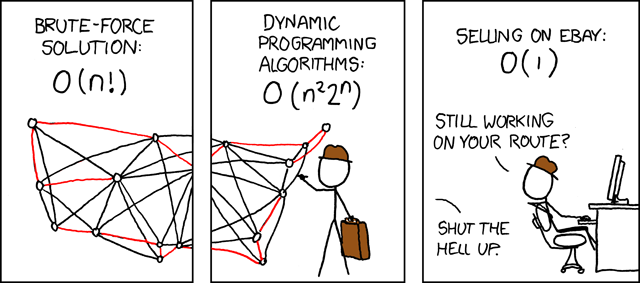
\includegraphics[width= \textwidth]{images/399_traveling_salesman}
		
		%\textit{\scriptsize{What's the complexity class of the best linear programming cutting-plane techniques? I couldn't find it anywhere. Man, the Garfield guy doesn't have these problems $\ldots$}}
		
		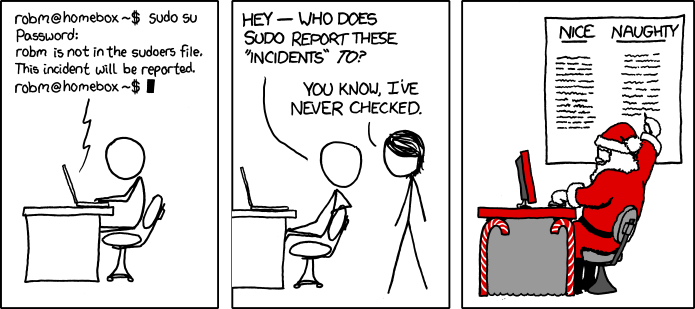
\includegraphics[width= \textwidth]{images/838_incident.png}
		
		\textit{\scriptsize{He sees you when you're sleeping, he knows when you're awake, he's copied on \texttt{/var/spool/mail/root}, so be good for goodness' sake.}}
		
	\end{figure}
\end{frame}

\frame{
  \frametitle{Lizenzen}
  \center
  \includegraphics[width=2em]{images/by}
  \includegraphics[width=2em]{images/cc}
  \includegraphics[width=2em]{images/sa}
  \\
  {\tiny

Dieses Werk ist unter einem ``Creative Commons Namensnennung-Weitergabe unter gleichen Bedingungen 3.0 Deutschland``-Lizenzvertrag lizenziert. Um eine Kopie der Lizenz zu erhalten, gehen Sie bitte zu \href{http://creativecommons.org/licenses/by-sa/3.0/de/}{http://creativecommons.org/licenses/by-sa/3.0/de/} oder schreiben Sie an Creative Commons, 171 Second Street, Suite 300, San Francisco, California 94105, USA.\\
  \vspace{1cm}
  Davon ausgenommen sind das Titelbild, welches aus der März-April 2002 Ausgabe von American Scientist erschienen ist und ohne Erlaubnis verwendet wird, sowie das KIT Beamer Theme. Hierfür gelten die Bestimmungen der jeweiligen Urheber.
  \vspace{1cm}
  \\ 
  }
  %Habe hier die Reihenfolge etwas umgestellt, weil die Formatierung bei mir komisch aussah. 
  %Wenn es bei dir anders ist, kannst du es auch wieder zurückändern, dann haben wir unterschiedliche Kompilieroptionen
}

\end{document}
